\documentclass[11pt]{article}
\usepackage{graphicx}
\usepackage[font=footnotesize, labelfont={sf,bf}, margin=1cm]{caption}
\usepackage{mathtools}
\usepackage{wrapfig}
\usepackage[letterpaper, portrait, margin=1in]{geometry}
\usepackage{framed}
\usepackage{listings}
\usepackage{color}
\usepackage{textcomp}
\usepackage[utf8]{inputenc}
\usepackage{pdfpages}
\definecolor{mauve}{rgb}{0.58,0,0.82}
\lstset{frame=tb,
  language=Lisp,
  aboveskip=3mm,
  belowskip=3mm,
  showstringspaces=false,
  columns=flexible,
  basicstyle={\small\ttfamily},
  numbers=none,
  numberstyle=\tiny\color{gray},
  keywordstyle=\color{blue},
  commentstyle=\color{cyan},
  stringstyle=\color{mauve},
  breaklines=true,
  breakatwhitespace=true,
  tabsize=3
}
%Gummi|065|=)
\title{\textbf{Implementing Associative Memory on a Quantum Computer Simulator}}
\author{William Bernoudy}
\date{}
\begin{document}

\maketitle

\begin{abstract}

This paper presents an implementation of associative memory on a quantum computer down to the gate level, using an algorithm by Ventura and Matinez. It gives an overview of the original algorithm as well as explains how the different components of the algorithm were accomplished using simple quantum gates. To illustrate this, the new algorithm is demonstrated by writing computer code for  quantum computer simulator.

\end{abstract}

\section{Introduction}

Associative memory deals with the problem of ``learning" a set of patterns, and then being able to ``recall" a certain pattern when presented with a part of the pattern. There are many simple classical algorithms that can achieve this task, such as storing the patterns in a database and then searching over the database (and each pattern) to find the one that matches. However, these can be slow and require lots of storage space. Another classical solution to this problem is using a Hopfield network, a type of neural network which can be trained with a set of patterns and then used to produce patterns when presented with a part of one. However, if the patterns are of length $n$, the neural network requires $n$ neurons, and is then limited in how many patterns it can store (usually less than half of $n$).

Quantum computing allows a significant improvement over neural network techniques. Dan Ventura and Tony Martinez, in a paper titled \textit{Quantum Associative Memory}, present two algorithms that achieve associative memory that allow up to $m=2^n$ patterns to be stored on $n$ qubits, with a training complexity of $O(mn)$ and a recall complexity of $O(\sqrt{n})$ \cite{Ven00}.

In order to show how this algorithm might actually be implemented on a universal quantum computer, each stage of Ventura's and Martinez's (V\&M) was achieved and simulated using only common quantum gates. Unless noted, all parts of the algorithms are taken directly from their paper.

\section{Explanation of Algorithms}

\subsection{Overview}

Given a set $P$ of patterns to be learned, each pattern is loaded one at a time onto the $n$ qubits until we have achieved an equal distribution of all the patterns. A slightly modified Grover's algorithm can then be used to retrieve a pattern based on a known portion of it.

\subsection{Learning Stage}

For patterns of length $n$, $n$ qubits are needed to store the pattern (called the storage qubits). However, during the learning stage, three extra qubits are necessary: 1 as an intermediate qubit which is always returned to $ \left | 0 \right \rangle$ ($g$), and two as control bits ($c_1$ and $c_2$). Note that this is a slight modification of V\&M's algorithm, which required $2n+2$ qubits. This is because I used a Z-gate with controls on every one of the storage bits for the sake of much shorter simulation times.\footnote{Any single qubit gate U with an arbitrary number of controls can be achieved by using a series of CNOT gates and twice the qubits.} For the algorithm, we require two special gates:

$$\mathrm{C0NOT}=\begin{pmatrix}
0 & 1 & 0 & 0 \\
1 & 0 & 0 & 0 \\
0 & 0 & 1 & 0 \\
0 & 0 & 0 & 1 \\
\end{pmatrix}$$

$$\mathrm{CS_p}=\begin{pmatrix}
1 & 0 & 0 & 0 \\
0 & 1 & 0 & 0 \\
0 & 0 & \sqrt{\frac{p-1}{p}} & \frac{-1}{\sqrt{p}} \\
0 & 0 & \frac{1}{\sqrt{p}} & \sqrt{\frac{p-1}{p}} \\
\end{pmatrix}$$

C0NOT is simply a controlled-not gate that flips the second bit if the first is zero, instead of one. It can be constructed by doing a NOT on the first qubit, a CNOT, and then another NOT on the first.

$\mathrm{CS_p}$ allows us to slice the state with the control bit as a one into two states, one being $\frac{1}{n}$ of the superposition, and the other being $\frac{p}{n}$ of the superposition.\footnote{A better and more in depth explanation of how this gate works can be found in V\&M's paper.}

Here are the steps of the algorithm for each pattern in $P$:

\begin{framed}
\textbf{Learning a single pattern on $n$ qubits:}
\begin{enumerate}
	\item Apply C0NOT gates with control on $c_2$ to storage qubit if the corresponding bit in the pattern is a 1.
	\item Apply C0NOT gate with control on $c_2$ to $c_1$.
	\item Apply $\mathrm{CS_p}$ with control on $c_1$ onto $c_2$, where $p$ is the number of patterns left including the pattern being learned.
	\item Apply NOT gates to every qubit where the corresponding bit in the pattern is a 0.
	\item Apply controlled NOT gate with controls on every storage qubit to $g$.
	\item Apply CNOT gate with control on $g$ to $c_1$.
	\item Repeat step 5.
	\item Repeat step 4.
\end{enumerate}
\end{framed}

We can repeat this algorithm for every pattern until $P$ has been ``learned" by the quantum computer. By the end of the algorithm, all three extra qubits, $g$, $c_1$ and $c_2$, will be unentangled from the rest of the system so we can safely discard them.

Note that is single pattern learning algorithm is $O(n)$, and as we must apply it for $m$ patterns, the entire learning algorithm is $O(mn)$.

\begin{figure}[!htb]
\centering
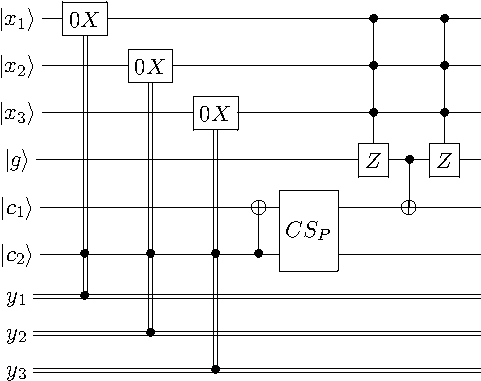
\includegraphics[width=0.5\textwidth]{assoc1-crop.pdf}
\caption{This example is for loading patterns with a length of 3. The pattern would come in loaded on the classical bits, $y_1$, $y_2$ and $y_3$. The 0X gate represents a controlled NOT except that the control looks for a zero on $c2$.}
\label{fig:digraph}
\end{figure}

\newpage

\subsection{Recall algorithm}

As previously stated, the recall algorithm uses a modified Grover search to find the correct learned pattern. The first difference is that we do not prepare the system in any way by applying Hadamard gates at the beginning, as we already have the superposition we want. The second is that at the beginning, since the Grover diffusion operator will also flip the phases of all the states representing the patterns (instead of just the desired pattern), we need another operator that flips all the phases of the patterns back. We call this operator $I_P$. In terms of the its matrix, it can be represented as an identity matrix where the $i$th 1 is changed to a $-1$ if $i$ is the decimal representation of one of the patterns. We can construct it with gates by going through every pattern, applying a NOT gate on the qubits that correspond to zeros in the pattern, applying a controlled Z with controls on every qubit (except the one with the Z-gate, which can be any of them), and then re-applying the same NOT gates. This method can be seen in the function \textit{constr-patterns-phaser} in my code. We will notate the normal Grover diffusion operator with $G$.

\begin{figure}[!htb]
\centering
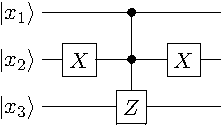
\includegraphics[width=0.25\textwidth]{assoc2-crop.pdf}
\caption{This example represents one pattern for $I_P$. The pattern would be (1 0 1), so we need to apply the NOT gate to the second qubit because it is a zero.}
\label{fig:digraph2}
\end{figure}

We want the oracle for Grover's algorithm to be a quantum circuit which flips the phase of the system if it is in the correct pattern. Thus, we can construct it simply by applying NOT gates to all qubits that correspond to zeros in the part of the pattern we know, applying a controlled Z gate with controls on all the qubits corresponding to bits we know onto one of the qubits corresponding to the qubits we don't know, and then applying the same NOT gates again. This method can be seen in the function \textit{constr-search-phaser} in my code. We will notate this oracle function with $I_s$.


\begin{figure}[!htb]
\centering
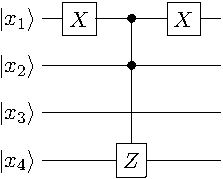
\includegraphics[width=0.25\textwidth]{assoc3-crop.pdf}
\caption{This example would correspond to the partial sequence (0 1 ? ?). We apply a NOT gate to the first qubit because we know it is a zero, then a Z with controls on the known qubits with a target on one of the unkowns, and then re-apply the NOT.}
\label{fig:digraph3}
\end{figure}

\begin{framed}
\textbf{Recalling pattern given partial sequence }
\begin{enumerate}
	\item Apply $I_sGI_PG$ to the qubits.
	\item Repeat $T$ times:
	\begin{enumerate}
		\item Apply $I_sG$ to the qubits.
	\end{enumerate}
	\item Measure register.
\end{enumerate}
\end{framed}

Where $$T=\frac{\frac{\pi}{2}-\arctan \left (\frac{k}{l}\sqrt{\frac{r_0+r_1}{N-r_0-r_1}} \right )}{\arccos \left ( 1-2\frac{r_0+r_1}{N} \right )}$$

and

$$k=4a-ab+\frac{r_1}{r_0+r_1}$$
$$l=-ab+\frac{2a(N+p-r_0-2r_1)}{N-r_0-r_1}-\frac{p-r_1}{N-r_0-r_1}$$
$$a=\frac{2(p-2r_1)}{N}$$
$$b=\frac{4(p+r_0)}{N}$$

and where $p$ is the number of patterns, $r_0$ is the number of marked states (states involving the unknown qubits that the controlled Z gates in $I_P$ did not act on, or, in the matrix representation, all the states corresponding to the $-1$s in the matrix) that do not correspond to learned patterns, and $r_1$ all the marked states that do correspond to learned states. In my code, I assumed that there was only one learned state that the recall should return, so I assumed $r_1$ is 1 and $r_0$ is equal to $2^u-1$ where $u$ is the number of unknowns in the partial sequence.\footnote{If you play around with a few more examples, you might notice that the code will not always produce the correctly matched string. This is covered in the conclusion.}

Though I have no understanding of $T$, V\&M assert that the second algorithm is still $O(\sqrt{n})$ and the same as Grover's algorithm. This makes sense in that though it was modified slightly, the algorithm remains essentially the same.

\section{qassoc.rkt}

\lstinputlisting{qassoc.rkt}

\subsection{Usage of Code}

The learning algorithm is called \textit{learn}, and the recall algorithm is called \textit{Grover-part}. You can use them like so:

\begin{lstlisting}
> (define P '((0 0 0 0) (0 0 1 1) (0 1 1 0) (1 0 0 1) (1 1 0 0) (1 1 1 1)))
> (learn P)
> (Grover-part '(0 1 1 ?) P)
> (measure-register)
The most likely result is |0110> with a probability of 0.8437500000000002
\end{lstlisting}

\section{Discussion and Conclusion}

Though in general I was able to successfully implement most parts of the algorithms outlined by V\&M, there was one notable issue that I had: The calculation of $T$ often gave me the wrong value. As a result, the code would often apply the oracle and Grover diffusion operator too many times and thus the final superposition was not likely to return the correct value. For example, when 6 patterns of length 4 are learned, and a partial sequence with two unknowns is used to recall, V\&M's definition of $T$ gives $T=3$. However, repeating the Grover step results in a final superposition with $\approx26\%$ chance of returning the wrong pattern, and only a $\approx9\%$ chance of retrieving the correct pattern. If we set $T=0$, however, the final system state has a $\approx84\%$ chance of returning the correct pattern. While this may be due to a mistake in my code or in my implementation of it, I have always been able to achieve a high rate of getting back the correct pattern using different values of $T$, which suggests there is an issue with my (or V\&M's) calculation of $T$.

\begin{thebibliography}{9}

	\bibitem{Ven00}
	Ventura, D., \& Martinez, T. (2000). Quantum associative memory. \emph{Information Sciences}, 124(1), 273-296.

\end{thebibliography}

\end{document}
